\documentclass[a4paper, 12pt]{article}
\usepackage[utf8]{inputenc}
\usepackage[bottom=3cm,top=2.5cm,left=2cm,right=2cm]{geometry}
\usepackage[brazil]{babel}
\usepackage{graphicx}
\usepackage{amsmath}
\usepackage{amssymb}
\usepackage{fancyhdr}
\usepackage{xcolor}
\fancyhf{}
\pagestyle{fancy}
\fancyfoot[LE,RO]{\thepage}
\setlength\headheight{26pt}
\rhead{
\includegraphics[width=4cm]{template-FEI/FEI_logo.png}}

\begin{document}
\noindent \textbf{Centro Universitário FEI}\\
\noindent \textbf{CC6112 - Computação Gráfica}\\
\noindent \textbf{Aluno: } João Pedro Rosa Cezarino  \\ 
\noindent \textbf{R.A: } 22.120.021-5\\
\\
\begin{center}
    \noindent \textbf{Resolução da Atividade 02 - Curvas e Superfícies}
\end{center}
\vspace{0.5cm}
\noindent\textbf{Questão 01:}\\
Plote os polinômios individuais da curva de Bézier de grau 2 sobre as mesmas coordenadas.
Responda onde cada polinômio exerce influência na curva de Bézier correspondente?\\
\\
\noindent\textbf{Solução:}
\\
$$P(t) = B_0.(1-t)^2 + 2,B_1 . t . (1-t) + B_2 . t^2$$
\begin{itemize}
\item\textbf{Para $t=0$:}
    \\
		$$B_0.(1)^2=B_0$$
		$$2.B_0.(1-t)=0$$
		$$B_2.0^2=0$$
\item\textbf{Para $t=1$:}
	\\
		$$B_0.(1-t)^2=0$$
		$$2.B_1.(1-t)=0$$
		$$B_2.1=B_2$$
	\\
\end{itemize}
\begin{minipage}[c]{0.5\linewidth} 
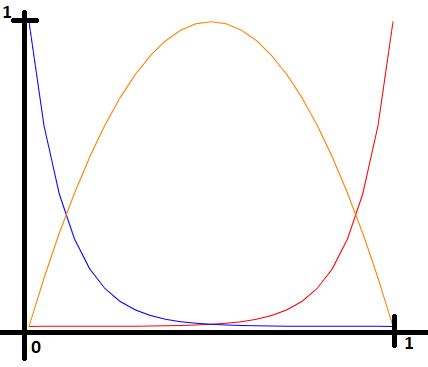
\includegraphics[width=\linewidth]{template-FEI/grafico.png}
\end{minipage}\hfill
\begin{minipage}[c]{0.4\linewidth} 
Observa-se que quando $t=0$, o valor de $B_0$ sobra na equação e portanto, não influencia no resultado. No caso de $t=1$, o valor de $B_2$ é o que sobra e também não influencia no resultado final. Nas situações restantes, todos os termos da equação influenciam no resultado final.
\end{minipage}

\vspace{1 cm}
\noindent\textbf{Questão 02:} \\
Sabemos que cada ponto de controle no polinômio de Bézier depende de todos os outros pontos.
Isso significa que, para construirmos uma curva com um número de pontos de controle muito
grande, como podemos construir tal curva somente com polinômios de grau 3?\\
\\
\noindent\textbf{Solução:}\\
Quanto mais pontos de controle presentes, mais as expressões ficarão complexas, isso pois, elas resultarão 
em polinômios de grau elevado. Para diminuir o grau desses polinômios, é possível conectar 
vários segmentos de curvas de graus menores, fazendo dois pontos que estejam conectados
por uma reta ter um ponto anterior ao final da curva e sobre ela.

\vspace{1 cm}
\noindent\textbf{Questão 03:}\\
Em um sistema com uma interface gráfica para construir curvas e superfícies, quais os parâmetros
mínimos necessários que um designer precisa fornecer ao sistema construir: a) uma curva de
Hermite; b) uma curva de Bézier\\
\\
\noindent\textbf{Solução:}
\begin{itemize}
    \item\textbf{a)} São necessários os pontos $P_1$ e $P_2$ e as tangentes $T_1$ e $T_2$.
    \item\textbf{b)} São necessários os pontos de controle de acordo com a equação de Bézier.
\end{itemize}

\vspace{1cm}
\noindent\textbf{Questão 04:}\\
Quais as diferenças básicas entre as curvas de Hermite, as curvas de Bézier e as B-Splines?\\
\\
\noindent\textbf{Solução:}
\\
Para as curvas de Hermite são usados dois pontos tangentes para formar uma curva. Já nas curvas de Bézier são usados pontos de controle que definem a forma da curva. Passando para as curvas B-splines, elas são uma generalização das curvas de Bézier, porém com mais propriedades e sem passar pelos pontos de controle, podem ser geradas para quaisquer números de ponto de controle. Com isso, o grau do polinômio fica independente do número de pontos de controle.

\vspace{1cm}
\noindent\textbf{Questão 05:}\\
Seja o Polinômio de Bézier: $P (t) = B0(1 − t)2 + 2B1t(1 − t) + B2t2$. Responda:
\begin{itemize}
\item \textbf{a)} Mostre o polinômio correspondente na forma racional, cujos pesos associados aos pontos de
controle $B0 = (2, 3)$, $B1 = (1, 0)$ e $B2 = (2, 1)$ são $w0 = 0.3$, $w1 = 0.5$, $w2 = 0.2$.
\item \textbf{b)} Qual o valor do Polinômio encontrado para $t = 0.5$ ?
\end{itemize}
\\
\noindent\textbf{Solução:}
\begin{itemize}
\item\textbf{a)} 
	\[
		\frac{W_0 \cdot B_0 \cdot (1-t)^2 + W_1 \cdot 2.B_1 \cdot t(1-t) + w_2 \cdot B_2 \cdot t^2}{W_0 \cdot (1-t)^2 + W_2 \cdot 2t \cdot (1-t) + w_2 \cdot t^2}
		\vspace{0.5cm}
	\]
	\[
	    \frac{W_0 \cdot (2, 3) \cdot (1-t)^2 + W_1 \cdot (1, 0) \cdot 2t(1-t) + w_2 \cdot (2, 1) \cdot t^2}{W_0 \cdot (1-t)^2 + W_2 \cdot 2t \cdot (1-t) + w_2 \cdot t^2}
		\vspace{0.5cm}
	\]
	\[
	    x(t) =
	    \frac{-0.2t + 0.6}{-0.5t^2 + 0.4t + 0.3}
	    \vspace{0.5cm}
	\]
	\[
	    y(t) =
	    \frac{1.1t^2 -1.8t + 0.9}{-0.5t^2 + 0.4t + 0.3}
	    \vspace{0.5cm}
	\]
	
\\
\item\textbf{b)}
    \[
        x(0.5) =
        \frac{-0.2 \cdot 0.5 + 0.6}{-0.5 \cdot 0.5^2 + 0.4 \cdot 0.5 + 0.3} = 1.333
        \vspace{0.5cm}
    \]
    \[
        y(0.5) =
        \frac{1.1 \cdot 0.5^2 - 1.8 \cdot 0.5 + 0.9}{-0.5 \cdot 0.5^2 + 0.4 \cdot 0.5 + 0.3} = 0.733
        \vspace{0.5cm}
    \]
    \[
         \therefore  \mathbf{P_w(0.5) = (1.33, 0.733)}
    \]
\end{itemize}
\vspace{1cm}
\noindent\textbf{Questão 06:}\\
Explique sucintamente como a utilização de curvas B-Splines pode ser vantajoso sobre as curvas
de Hermite ou Bezier, para aplicações que usam movimentação de câmeras, como no caso de
jogos online. Por exemplo, para navegar um humanóide ou avatar no ambiente imerso.\\
\\
\noindent\textbf{Solução:}
\\
As curvas \textbf{B-splines} possuem a vantagem de não depender exclusivamente dos pontos de controle, diferentemente das curvas de Bézier. Dessa forma, as mudanças de câmera possuem uma transição mais suave e uniforme.

\vspace{1cm}
\noindent\textbf{Questão 07:}\\
Abaixo são dadas duas curvas paramétricas (Hermite e Bézier), não necessariamente nessa ordem.
Os pontos de controle utilizados são o vetor $[B0, B1, B2, B3]$. No caso da curva de Hermite, $B2$ e $B3$
são as tangentes associadas aos pontos $B0$ e $B1$, respectivamente. Nessas curvas, $t = [0:1]$ é o
parâmetro de avaliação das curvas e o símbolo $’$ significa transposto. Supomos $B0 = (1,1)$, $B1 = (4,3)$,
$B2 = (6,2)$ e $B3 = (8,1)$. Responda as questões que virão na seqüência.
$$P(t) = [(2t^3-3t^2+1) \ (-2t^3+3t^2) \ (t^3-2t^2+t) \ (t^3-t^2) ] \ [B0, B1, B2, B3]’$$
$$P(t) = [(-t^3+3t^2-3t+1) \ (3t^3-6t^2+4) \ (-3t^3+3t^2+3t+1) \ (t^3)] \ [B0, B1, B2, B3]’$$
\begin{itemize}
\item \textbf{1.1)} Tomando a curva de Hermite como referência, qual o polinômio na primeira dimensão quando o
valor do parâmetro $t = 0.3$? Como você reconheceu a curva de Hermite?
\item \textbf{1.2)} Tomando a curva de Bézier como referência, considere o vetor de pesos $[w0, w1, w2, w3]$
associados aos quanto pontos de controle dados. Se inicialmente $w0 = w1 = w2 = w3 = 1.0$, qual o
valor que devemos atribuir a um dos pesos para que a curva se aproxime do ponto $B_1$ 50\% da
distância atual?
\end{itemize}
\\
\noindent\textbf{Solução:}
\begin{itemize}
\item\textbf{1.1)}
\begin{center}
    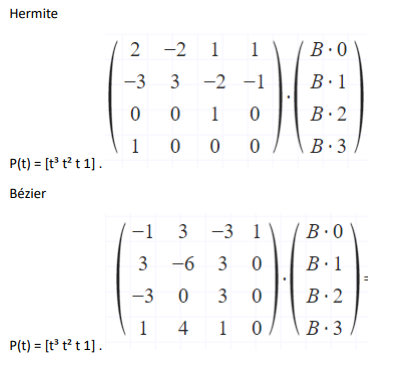
\includegraphics[]{template-FEI/sete01.png}
\end{center}
Tomando por base a expressão obtida acima, a curva de Hermite é a primeira equação, pois se decompô-la chegaremos na formula de Hermite.
\begin{center}
    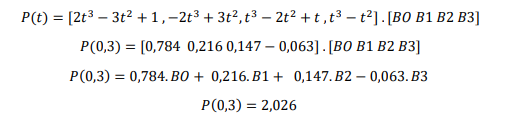
\includegraphics[]{template-FEI/sete02.png}
\end{center}
\vspace{0.5cm}
\item\textbf{1.2)}
\[
	P(t)=\frac{W_1.(1-t)^3.B_0+W_2.3.t.(1-t)^2.B_1+W_3.3t^2.(1-t).B_2+W_4.t^3.B_3}{W_1.(1-t)^3+W_2.3.t.(1-t)^2+W_3.3.t^2.(1-t)+W_4.t^3}
	\vspace{0.5cm}
\]
\text{Para aproximar 50\% de} $B_1$ \text{devemos alterar o peso de} $W_2$.
\\
\[\therefore \mathbf{W_2 = 1,5}\]
\end{itemize}

\vspace{1cm}
\noindent\textbf{Questão 08:}\\
Considere os seguintes pontos de controle que definem uma curva de Bezier: $B0 = (0,2)$, $B1 = (1,-2)$, $B2 = (3,0)$,
$B3 = (4,3)$. Responda as questões abaixo:
\begin{itemize}
\item\textbf{a)} Escreva as equações paramétricas $x(t)$ e $y(t)$.
\item\textbf{b)} Determine os pontos da curva que correspondem a $t=0.1$ e $t=0.6$.
\item\textbf{c)} Represente graficamente a curva.
\item\textbf{d)} Trace, sobre o gráfico da curva, o seu Convex Hull.
\end{itemize}
\\
\\
\noindent\textbf{Solução:}
\begin{itemize}
\item\textbf{a)}
\[P_x(t) = (1-t)^3.B_0x+3.t.(1-t)^2.B_1x+3.t^2.(1-t).B_2x+t^2.B_3x
\vspace{0.5cm}\]
\[P_x(t) = (1-t)^3.0+3.t.(1-t)^2.1+3.t^2.(1-t).3+t^3.4
\vspace{0.5cm}\]
\[P_x(t) = 3.t.(1-t)^2+9.t^2.(1-t)+4.t^3
\vspace{0.5cm}
\]
\[P_y(t) = (1-t)^3.B0y+3.t.(1-t)^2.B1y+3.t^2.(1-t).B2y+t^3.B3y
\vspace{0.5cm}\]
\[P_y(t) = (1-t)^3.2+3.t.(1-t)^2.-2+3.t^2.(1-t).0+t^3.3
\vspace{0.5cm}\]
\[P_y(t) = 2.(1-t)^3-6.t.(1-t)^2+3.t^3
\vspace{0.5cm}
\]
\item\textbf{b)}

\[P_x(t) = 3.t.(1-t)^2+9.t^2.(1-t)+4.t^3
\vspace{0.5cm}\]
\[P_y(t) = 2.(1-t)^3-6.t.(1-t)^2+3.t^3
\vspace{0.5cm}
\]
\[P_x=(0,1)
\
\]
\[P_y=(0,6)
\vspace{0.5cm}
\]
\[P_x(0.1) = 3.0,1.(1-0,1)^2+9.0,1^2.(1-0,1)+4.0,1^3
\vspace{0.5cm}\]
\[P_x(0.1) = 0.328
\vspace{0.5cm}\]
\[P_y(0.1) = 2.(1-0,1)^3-6.0,1.(1-0,1)^2+3.0,1^3
\vspace{0.5cm}\]
\[P_y(0.1) = 0.975
\vspace{0.5cm}
\]
\[P_x(0.6) = 3.0,6.(1-0,6)^2+9.0,6^2.(1-0,6)+4.0,6^3
\vspace{0.5cm}\]
\[P_x(0.6) = 2.448
\vspace{0.5cm}
\]
\[P_y(0.6) = 2.(1-0,6)^3-6.0,6.(1-0,6)^2+3.0,6^3
\vspace{0.5cm}\]
\[P_y(0.6) = 0.2
\vspace{0.5cm}\]
\item\textbf{c)}
\begin{center}
   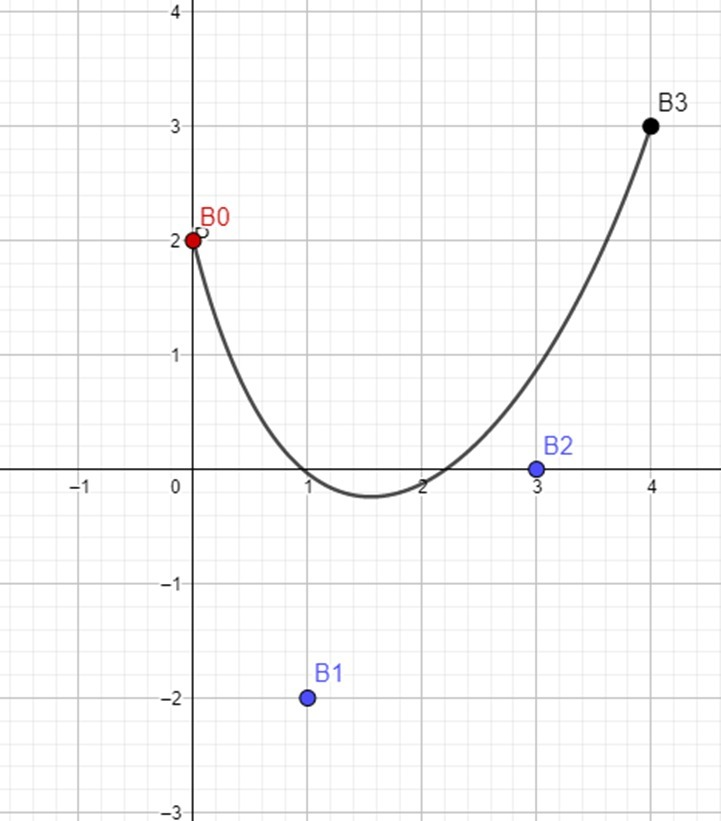
\includegraphics[width=8cm, height=8cm]{template-FEI/oitoc.jpeg} 
\end{center}
\item\textbf{d)}
\begin{center}
   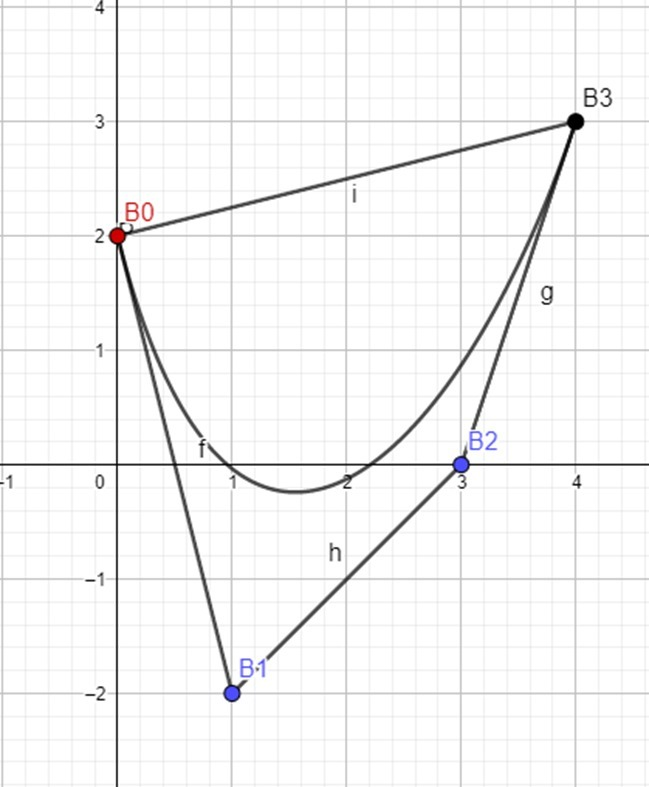
\includegraphics[width=8cm, height=8cm]{template-FEI/oitod.jpeg} 
\end{center}
\vspace{0.5cm}
\vspace{0.5cm}
\end{itemize}
\end{document}
